\newpage
\section[Фигура 4]{Фигура 4}

Строим круг и зведу, используя примитивы \textbf{Inkscape}. 
Применяем выравнивание.
Последовательно применяем операции 
\textit{\textbf{Duplicate, Exclusion, Division, Delete}}.
Производим заливку фигуры, инструмент \textit{\textbf{Fill and Stroke}}.
\begin{figure}[H]
    \begin{minipage}[h]{0.25\linewidth}
        \center{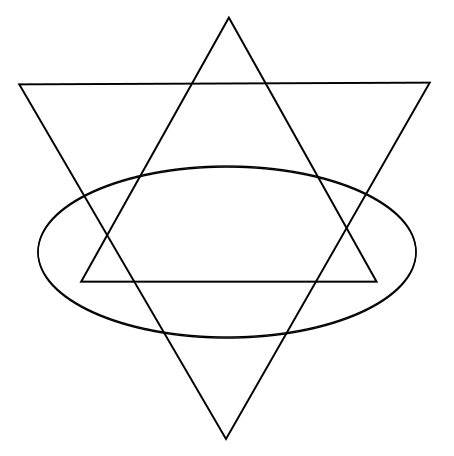
\includegraphics[width=1\linewidth]{4_1_create.png}}\\Создание фигур
    \end{minipage}
    \hfill
    \begin{minipage}[h]{0.25\linewidth}
        \center{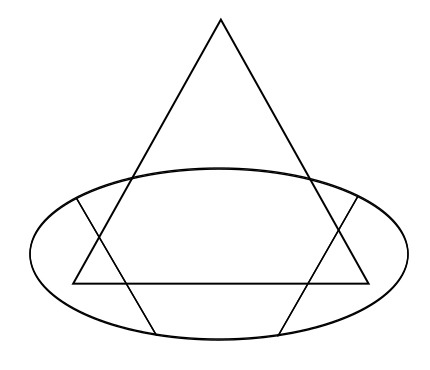
\includegraphics[width=1\linewidth]{4_2_division.png}}\\Division
    \end{minipage}
    \hfill
    \begin{minipage}[h]{0.25\linewidth}
        \center{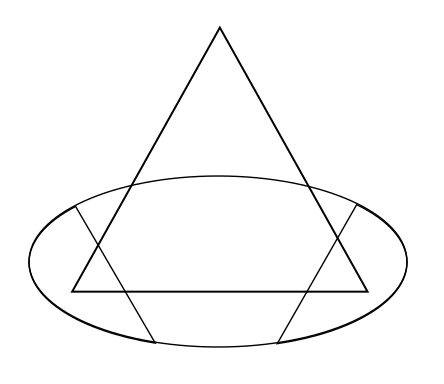
\includegraphics[width=1\linewidth]{4_3_delete.png}}\\Delete\\
    \end{minipage}
    \vfill
    \vspace*{1cm}
    \begin{minipage}[h]{0.25\linewidth}
        \center{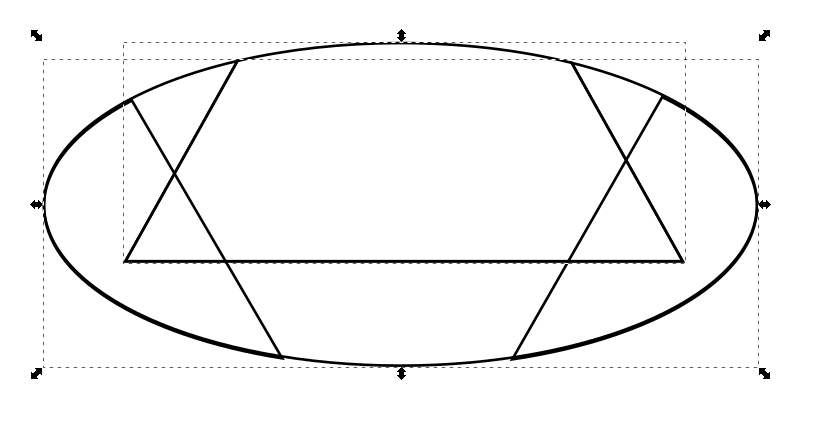
\includegraphics[width=1\linewidth]{4_4_division.png}}\\Division
    \end{minipage}    
    \hfill
    \begin{minipage}[h]{0.25\linewidth}
        \center{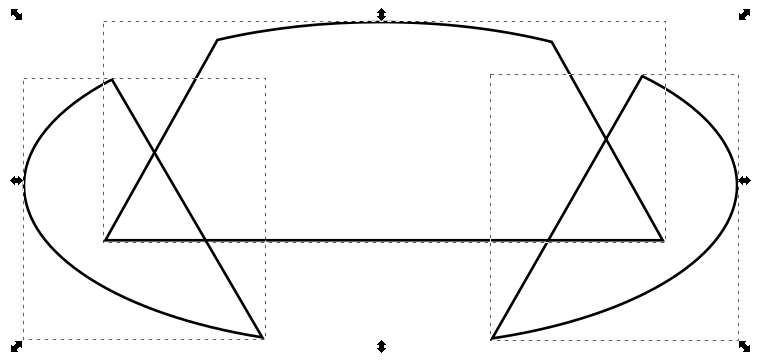
\includegraphics[width=1\linewidth]{4_5_delete.png}}\\Delete
    \end{minipage}
    \hfill
    \begin{minipage}[h]{0.25\linewidth}
        \center{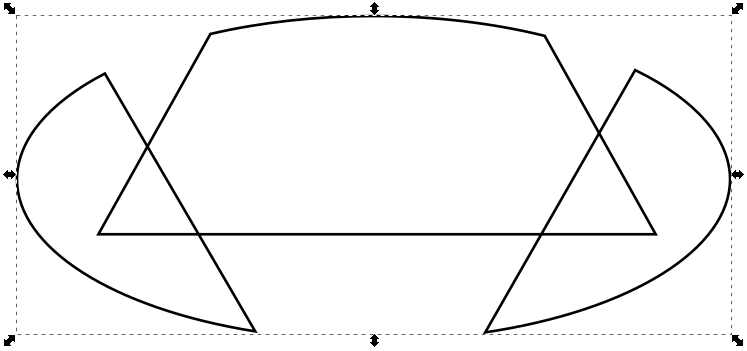
\includegraphics[width=1\linewidth]{4_6_exclusion.png}}\\Exclusion
    \end{minipage}
    \vfill
    \vspace*{1cm}
    \centering
    \begin{minipage}[h]{0.25\linewidth}
        \center{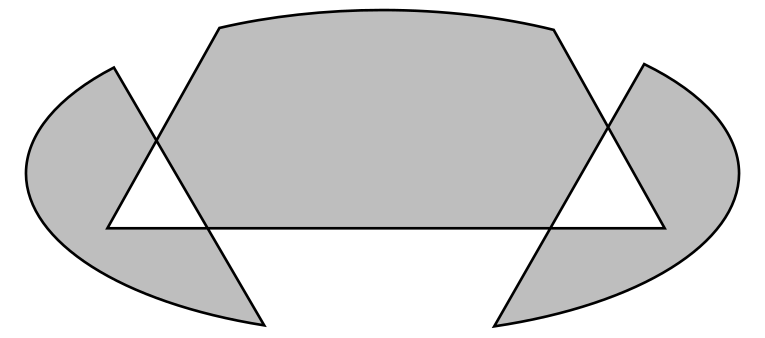
\includegraphics[width=1\linewidth]{4_7_fill.png}}\\Fill and Stroke
    \end{minipage}
\end{figure}
